\documentclass[12pt,a4paper]{article}
\usepackage[utf8]{inputenc}
\usepackage[english]{babel}
\usepackage[english]{isodate}
\usepackage[parfill]{parskip}
\usepackage{filecontents,listings}


\usepackage{geometry}
 \geometry{
 a4paper,
 total={170mm,257mm},
 left=20mm,
 top=20mm,
 }


\usepackage{framed}
\usepackage{hyperref}
\usepackage{todonotes}
\usepackage{graphicx}
\usepackage{xcolor}
\usepackage{color}
% define colors for source code list
\definecolor{colKeys}{rgb}{0,0,1}
\definecolor{colIdentifier}{rgb}{0,0,0}
\definecolor{colComments}{rgb}{0,1,0.3}
\definecolor{colString}{rgb}{0,0.5,0}

\definecolor{dkgreen}{rgb}{0,0.6,0}
\definecolor{gray}{rgb}{0.5,0.5,0.5}
\lstset{
   keywords={break,case,catch,continue,else,elseif,end,for,function,
   global,if,otherwise,persistent,return,switch,try,while,ones,zeros},
   float=hbp,
   basicstyle=\ttfamily\scriptsize,
   identifierstyle=\color{colIdentifier},
   %keywordstyle=\color{blue},
   commentstyle=\color{red},
   stringstyle=\color{dkgreen},
   columns=flexible,
   tabsize=2,
   frame=single,
   numbers=left,
   extendedchars=true,
   showspaces=false,
   numberstyle=\tiny\color{gray},
   stepnumber=1,
   numbersep=10pt,
   showspaces=false,
   showstringspaces=false,
   breakautoindent=true,
   breaklines=true}
   \renewcommand{\rmdefault}{phv} % Arial
\renewcommand{\sfdefault}{phv} % Arial
\begin{document}


\pagenumbering{Roman}
\begin{titlepage}
\pagecolor{black}
\vspace*{\fill}
		%\raggedleft\textbf{\Huge Molecular-Toolbox}\\
		\centering 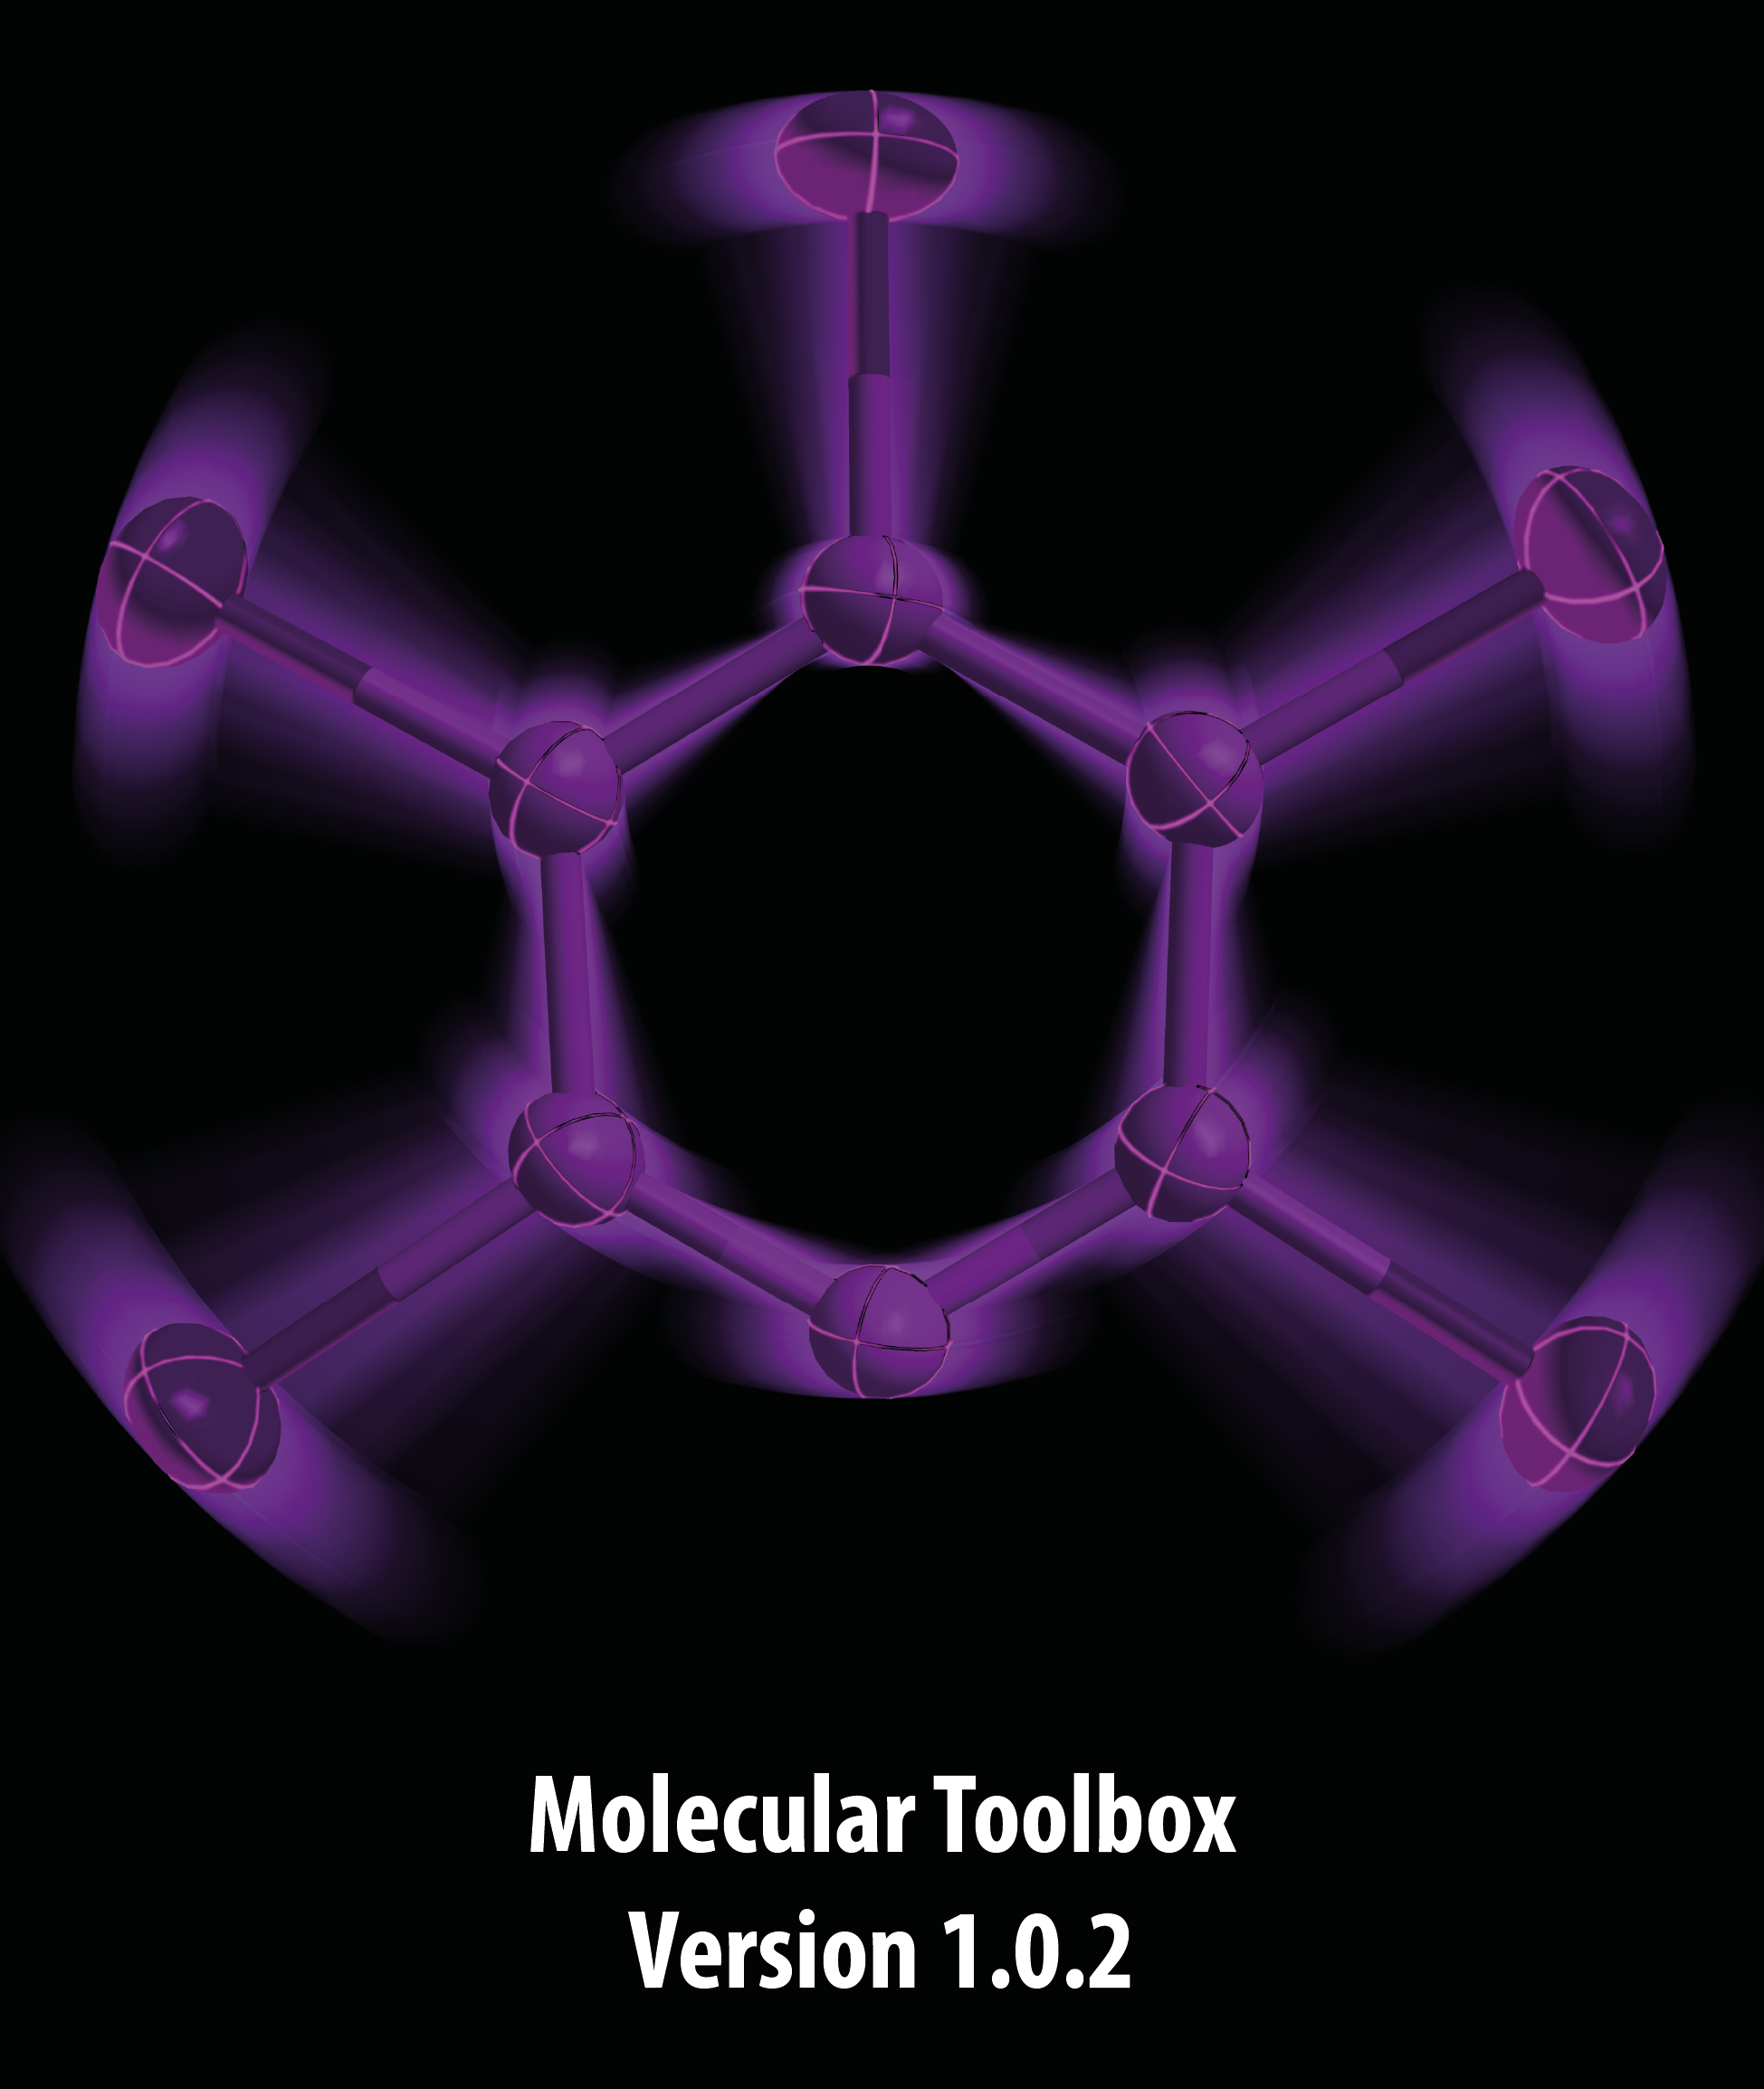
\includegraphics[width=1.0\textwidth]{Unbenannt-1-01.png}
		\vfill

\end{titlepage}
\pagecolor{white}
\vfill
\raggedright\textbf{\Large  The Dronskowski Group at RWTH Aachen University, Aachen, Germany, proudly presents:}\\
\vfill
		%\raggedleft\textbf{\Huge Molecular-Toolbox}\\
		\centering 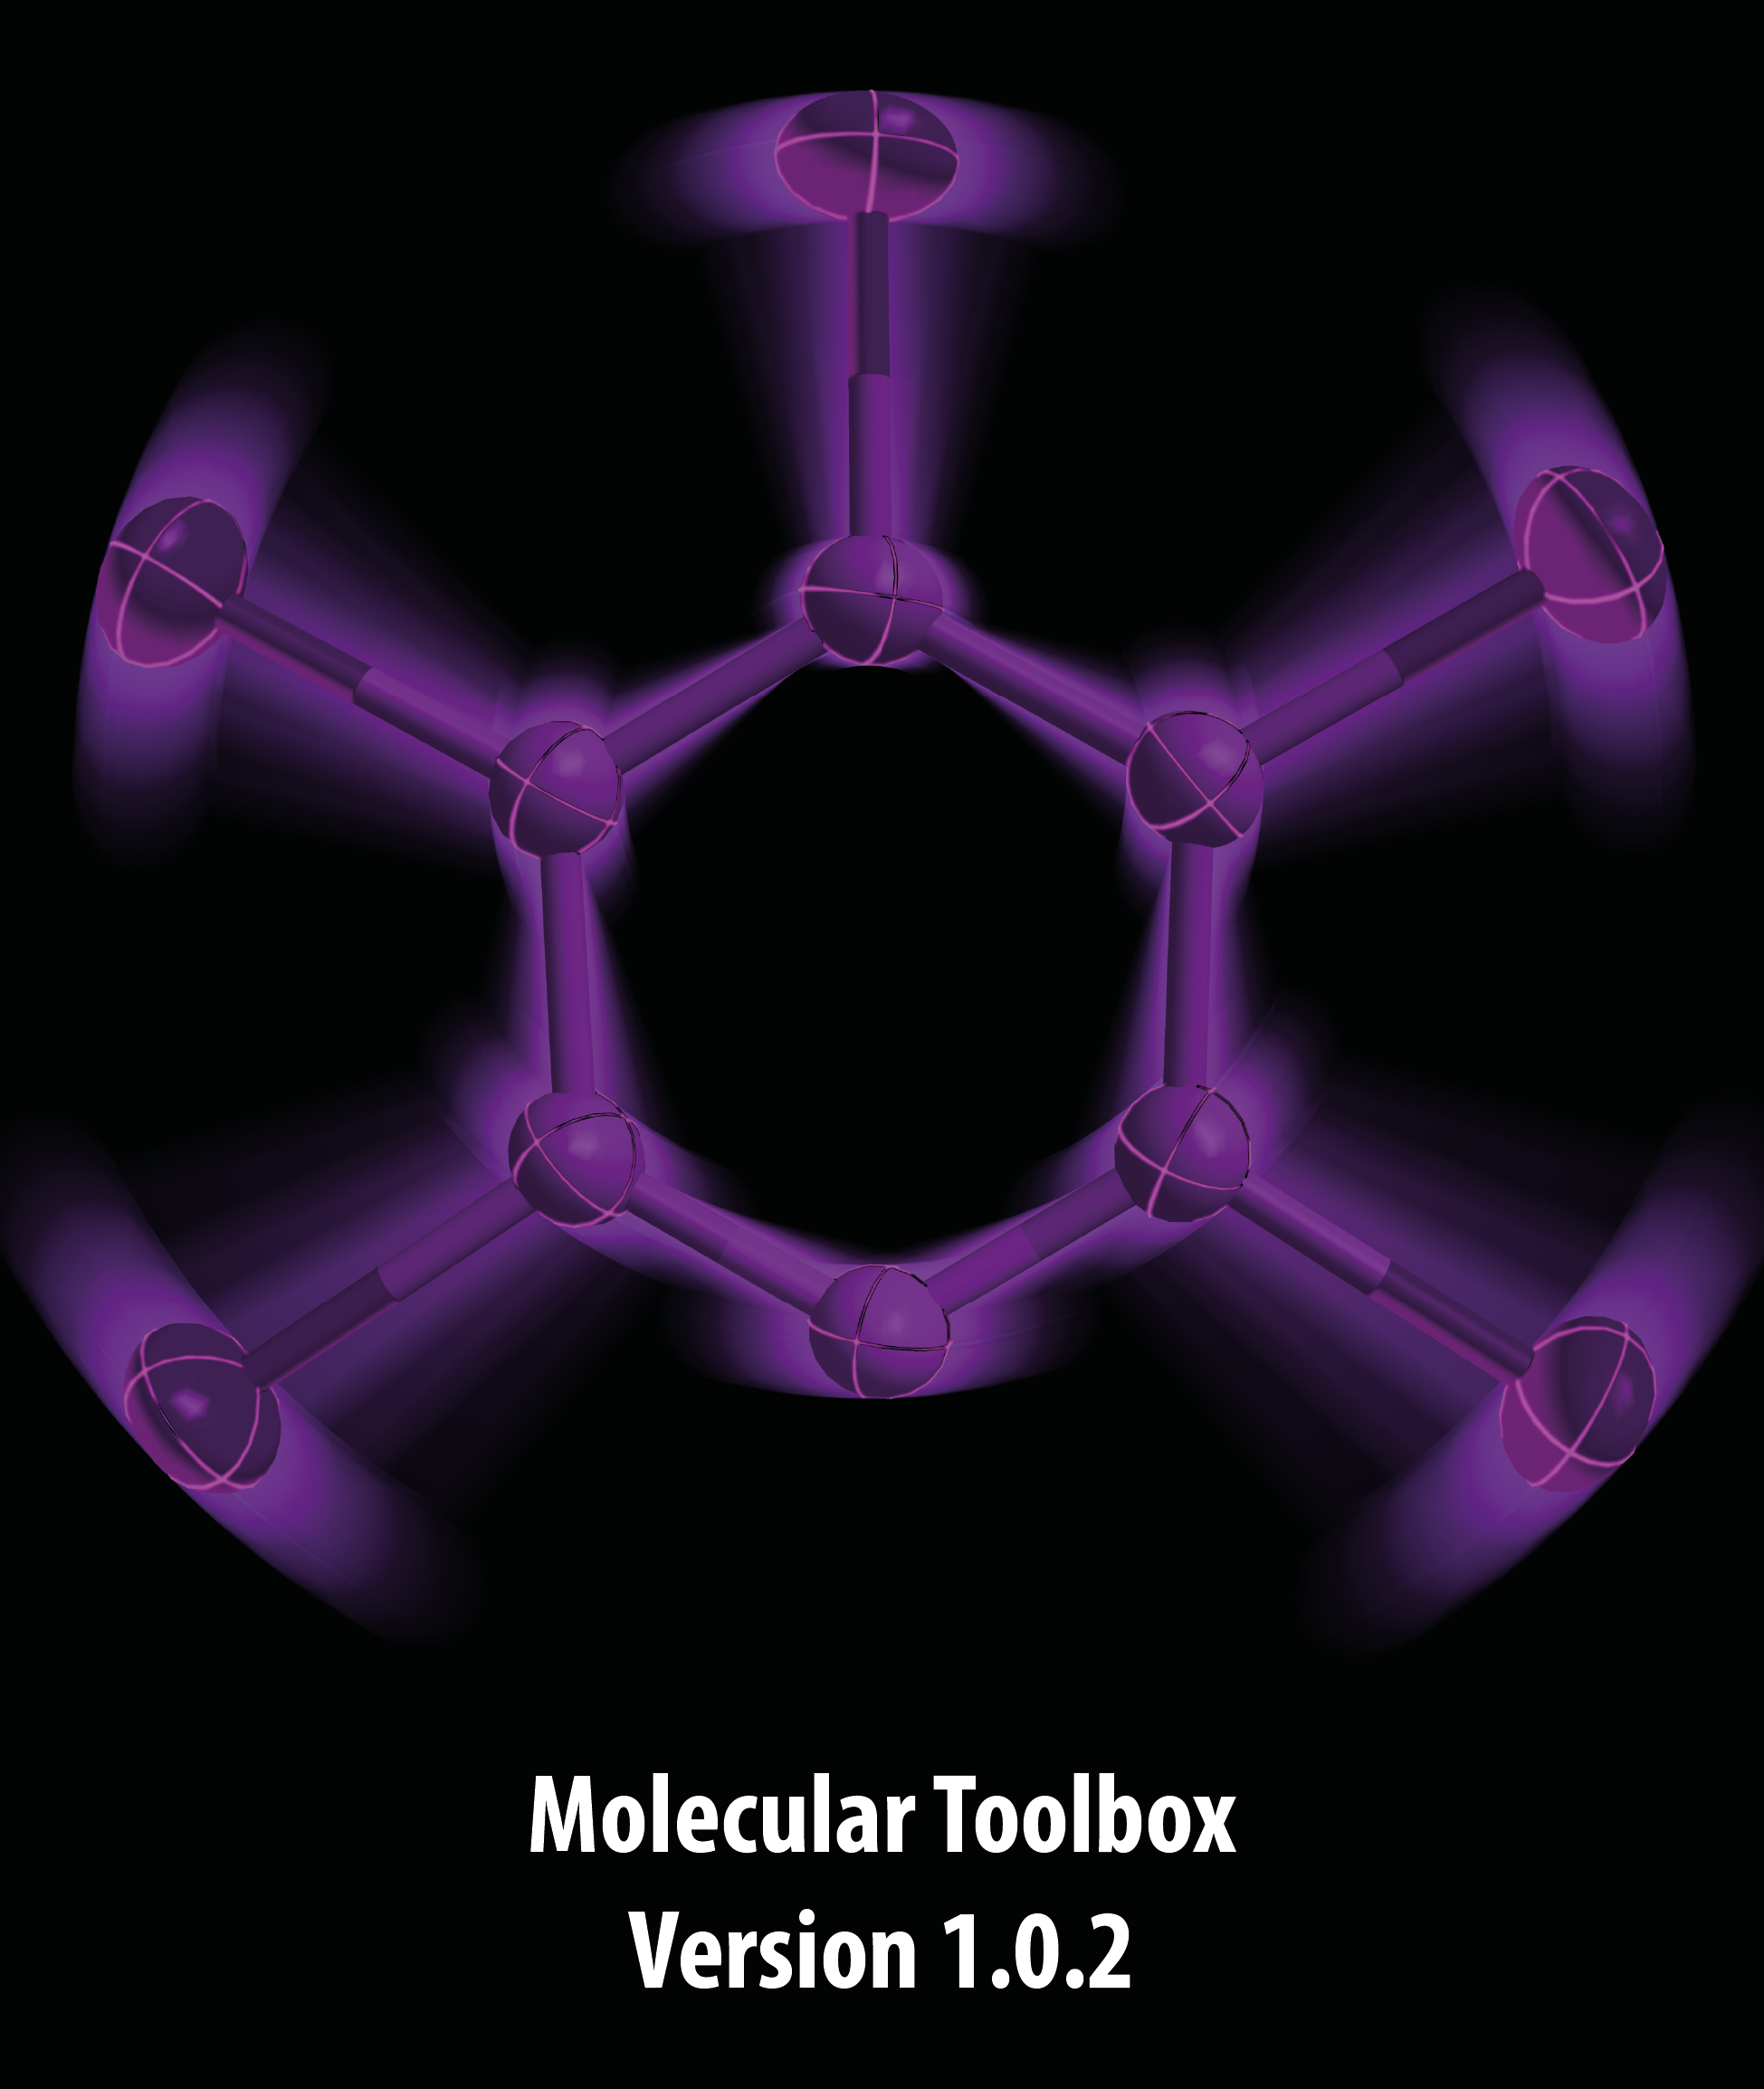
\includegraphics[width=1.0\textwidth]{Unbenannt-1-01.png}
		\vfill
\raggedright\textbf{\Large Copyright \copyright 2015--2017, Aachen, Germany.}
\vfill
\newpage




\tableofcontents
\newpage
\pagenumbering{arabic}


\section{Introduction}
\subsection{Features of the Toolbox}


\textbf{1. Conversion of Anisotropic Displacement Parameters to Different Parametrizations}\\
\begin{center}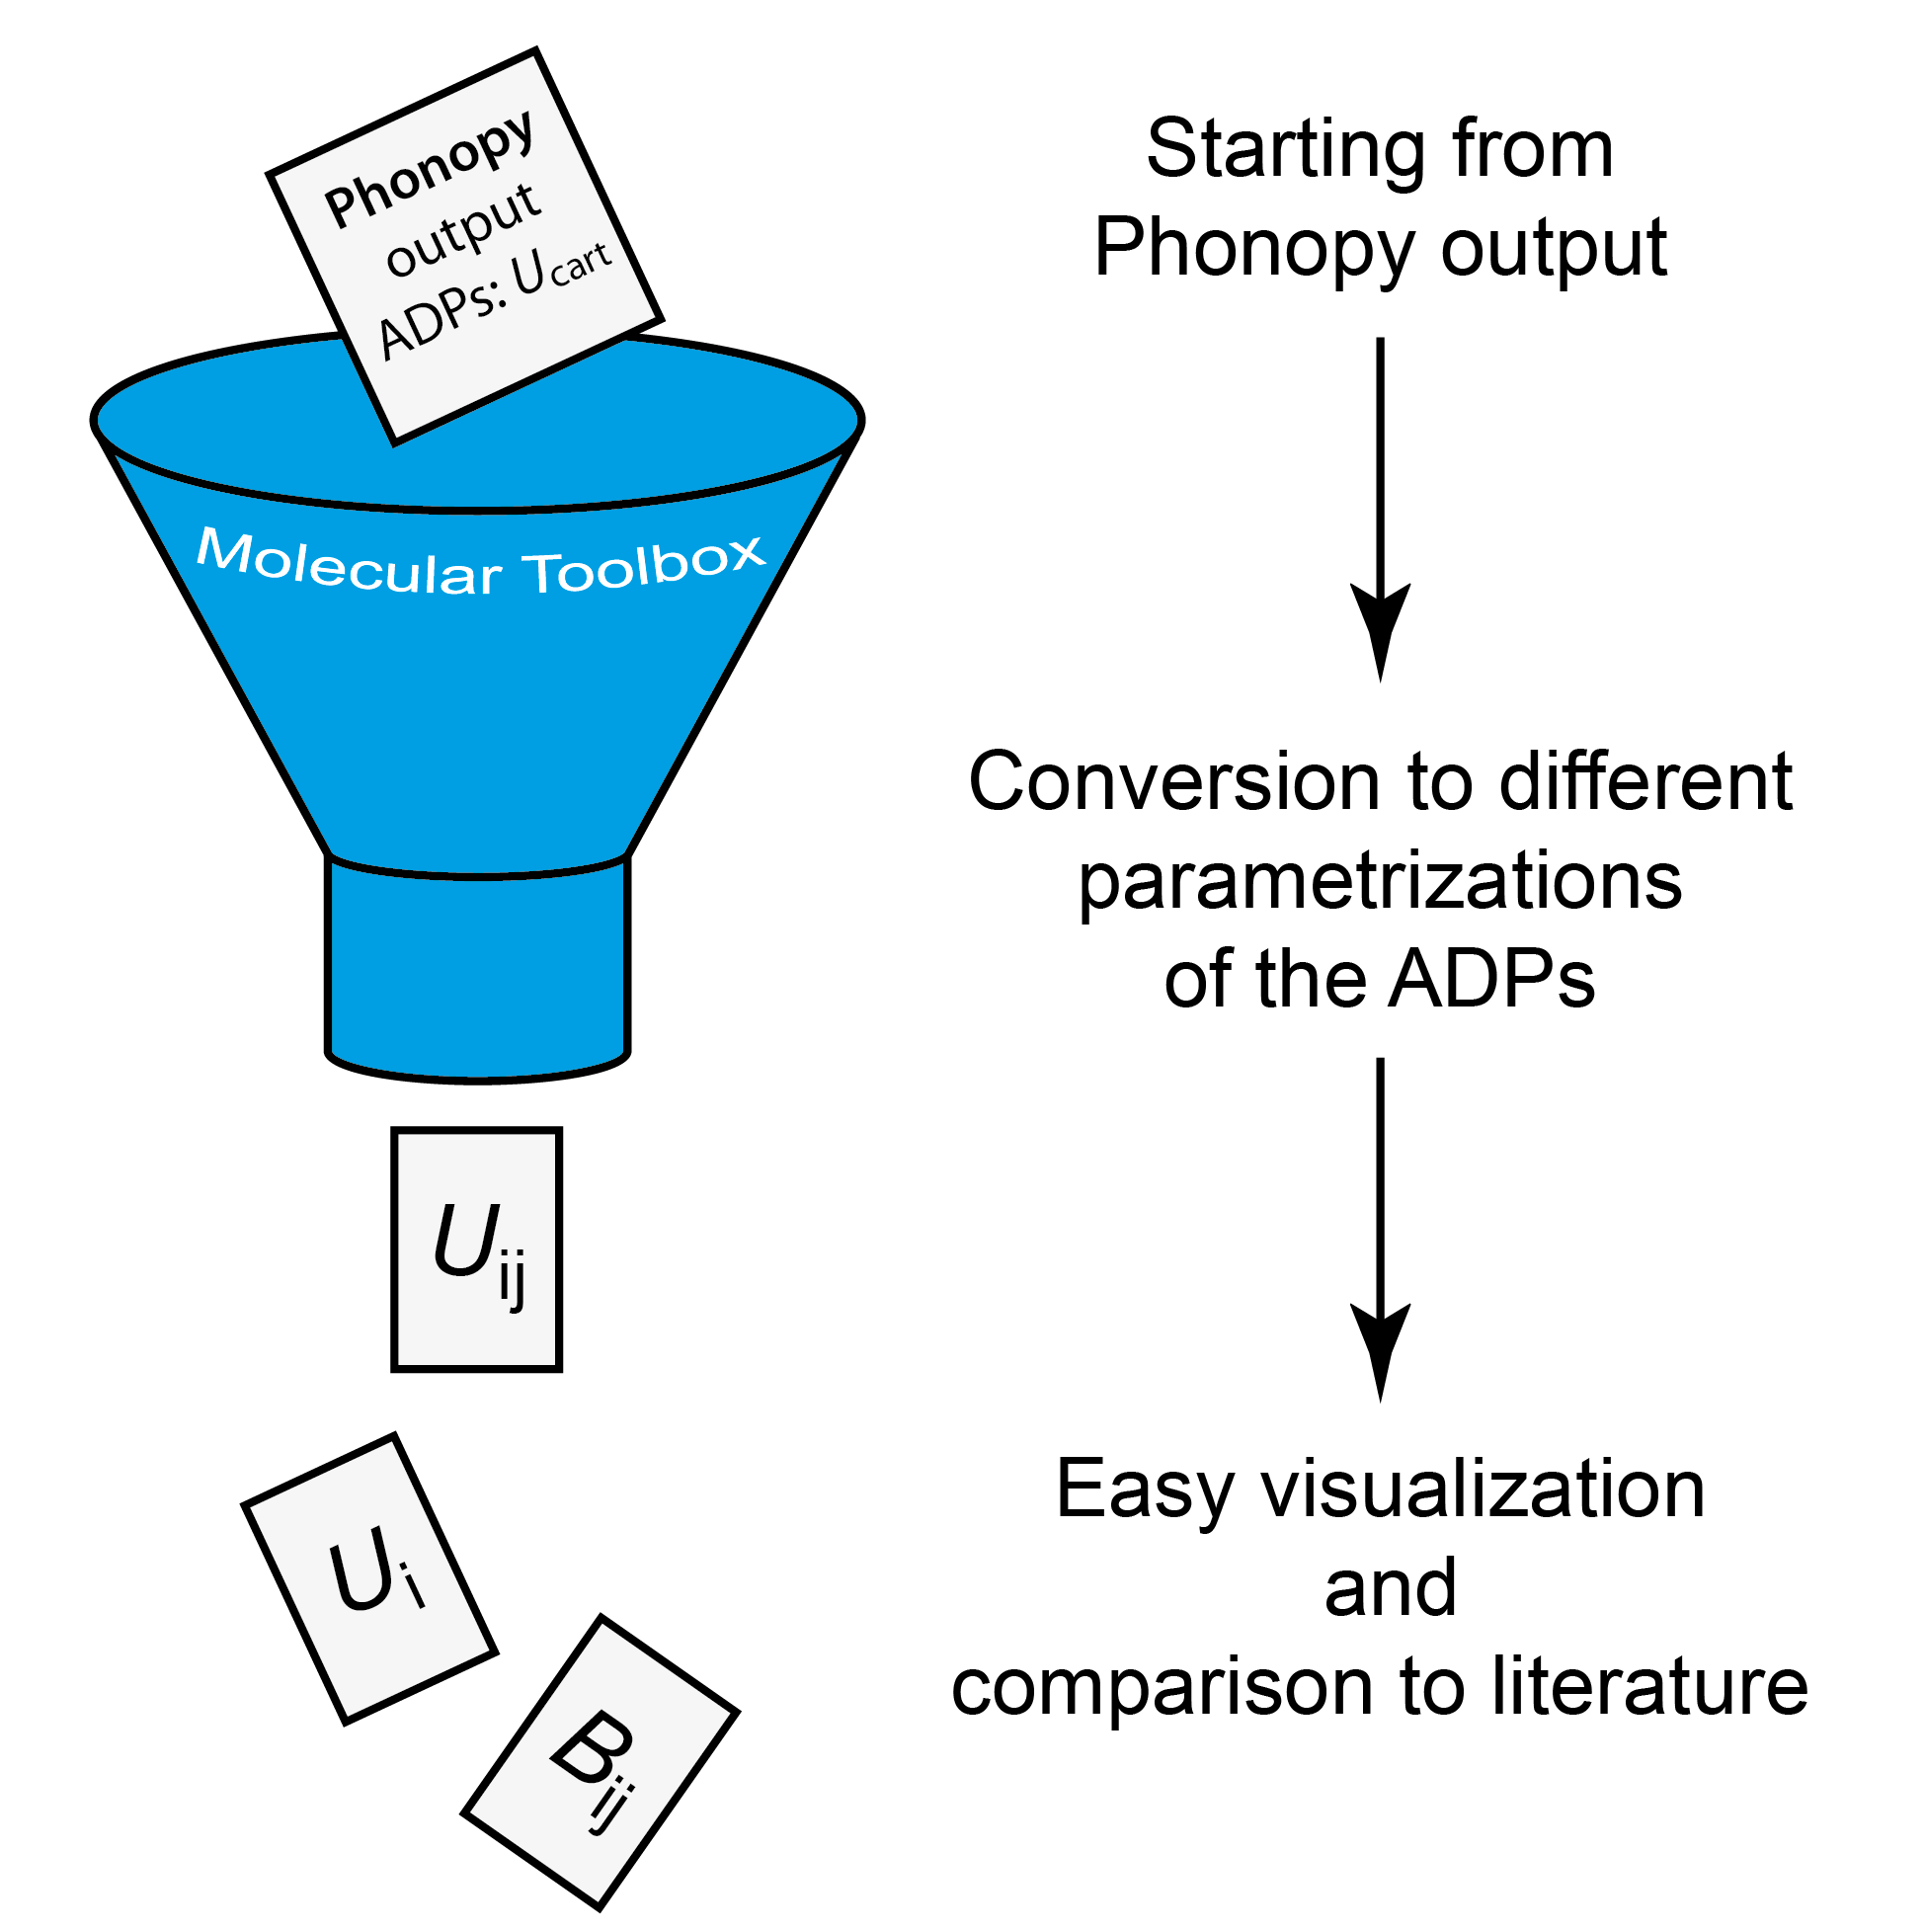
\includegraphics[width=0.4\textwidth]{Piktogramm-01.png}\end{center}


This toolbox can convert anisotropic displacement parameters calculated with \href{http://phonopy.sourceforge.net/}{Phonopy} referring to a Cartesian coordinate system ($U_{\mathrm{cart}}$) to $U_{\mathrm{cif}}$, $B$, $U^\mathrm{*}$, $\beta$, $U_{i}$ and $U_{\mathrm{eq}}$. Moreover, $U_{\mathrm{cif}}$, $B$, $U^\mathrm{*}$ and $\beta$ from literature can be converted to $U_{\mathrm{cif}}$, $B$, $U^\mathrm{*}$ and $\beta$. 

This is all done according to:\\ R. W. Grosse-Kunstleve and P. D. Adams, \textit{J. Appl. Crystallogr.}, \textbf{2002}, \textit{35}, 477–480.\\ This article also includes the nomenclature of the different parametrizations.

\textbf{2. Calculation of the Root-Mean-Square of the Cartesian Displacements}\\

\begin{center}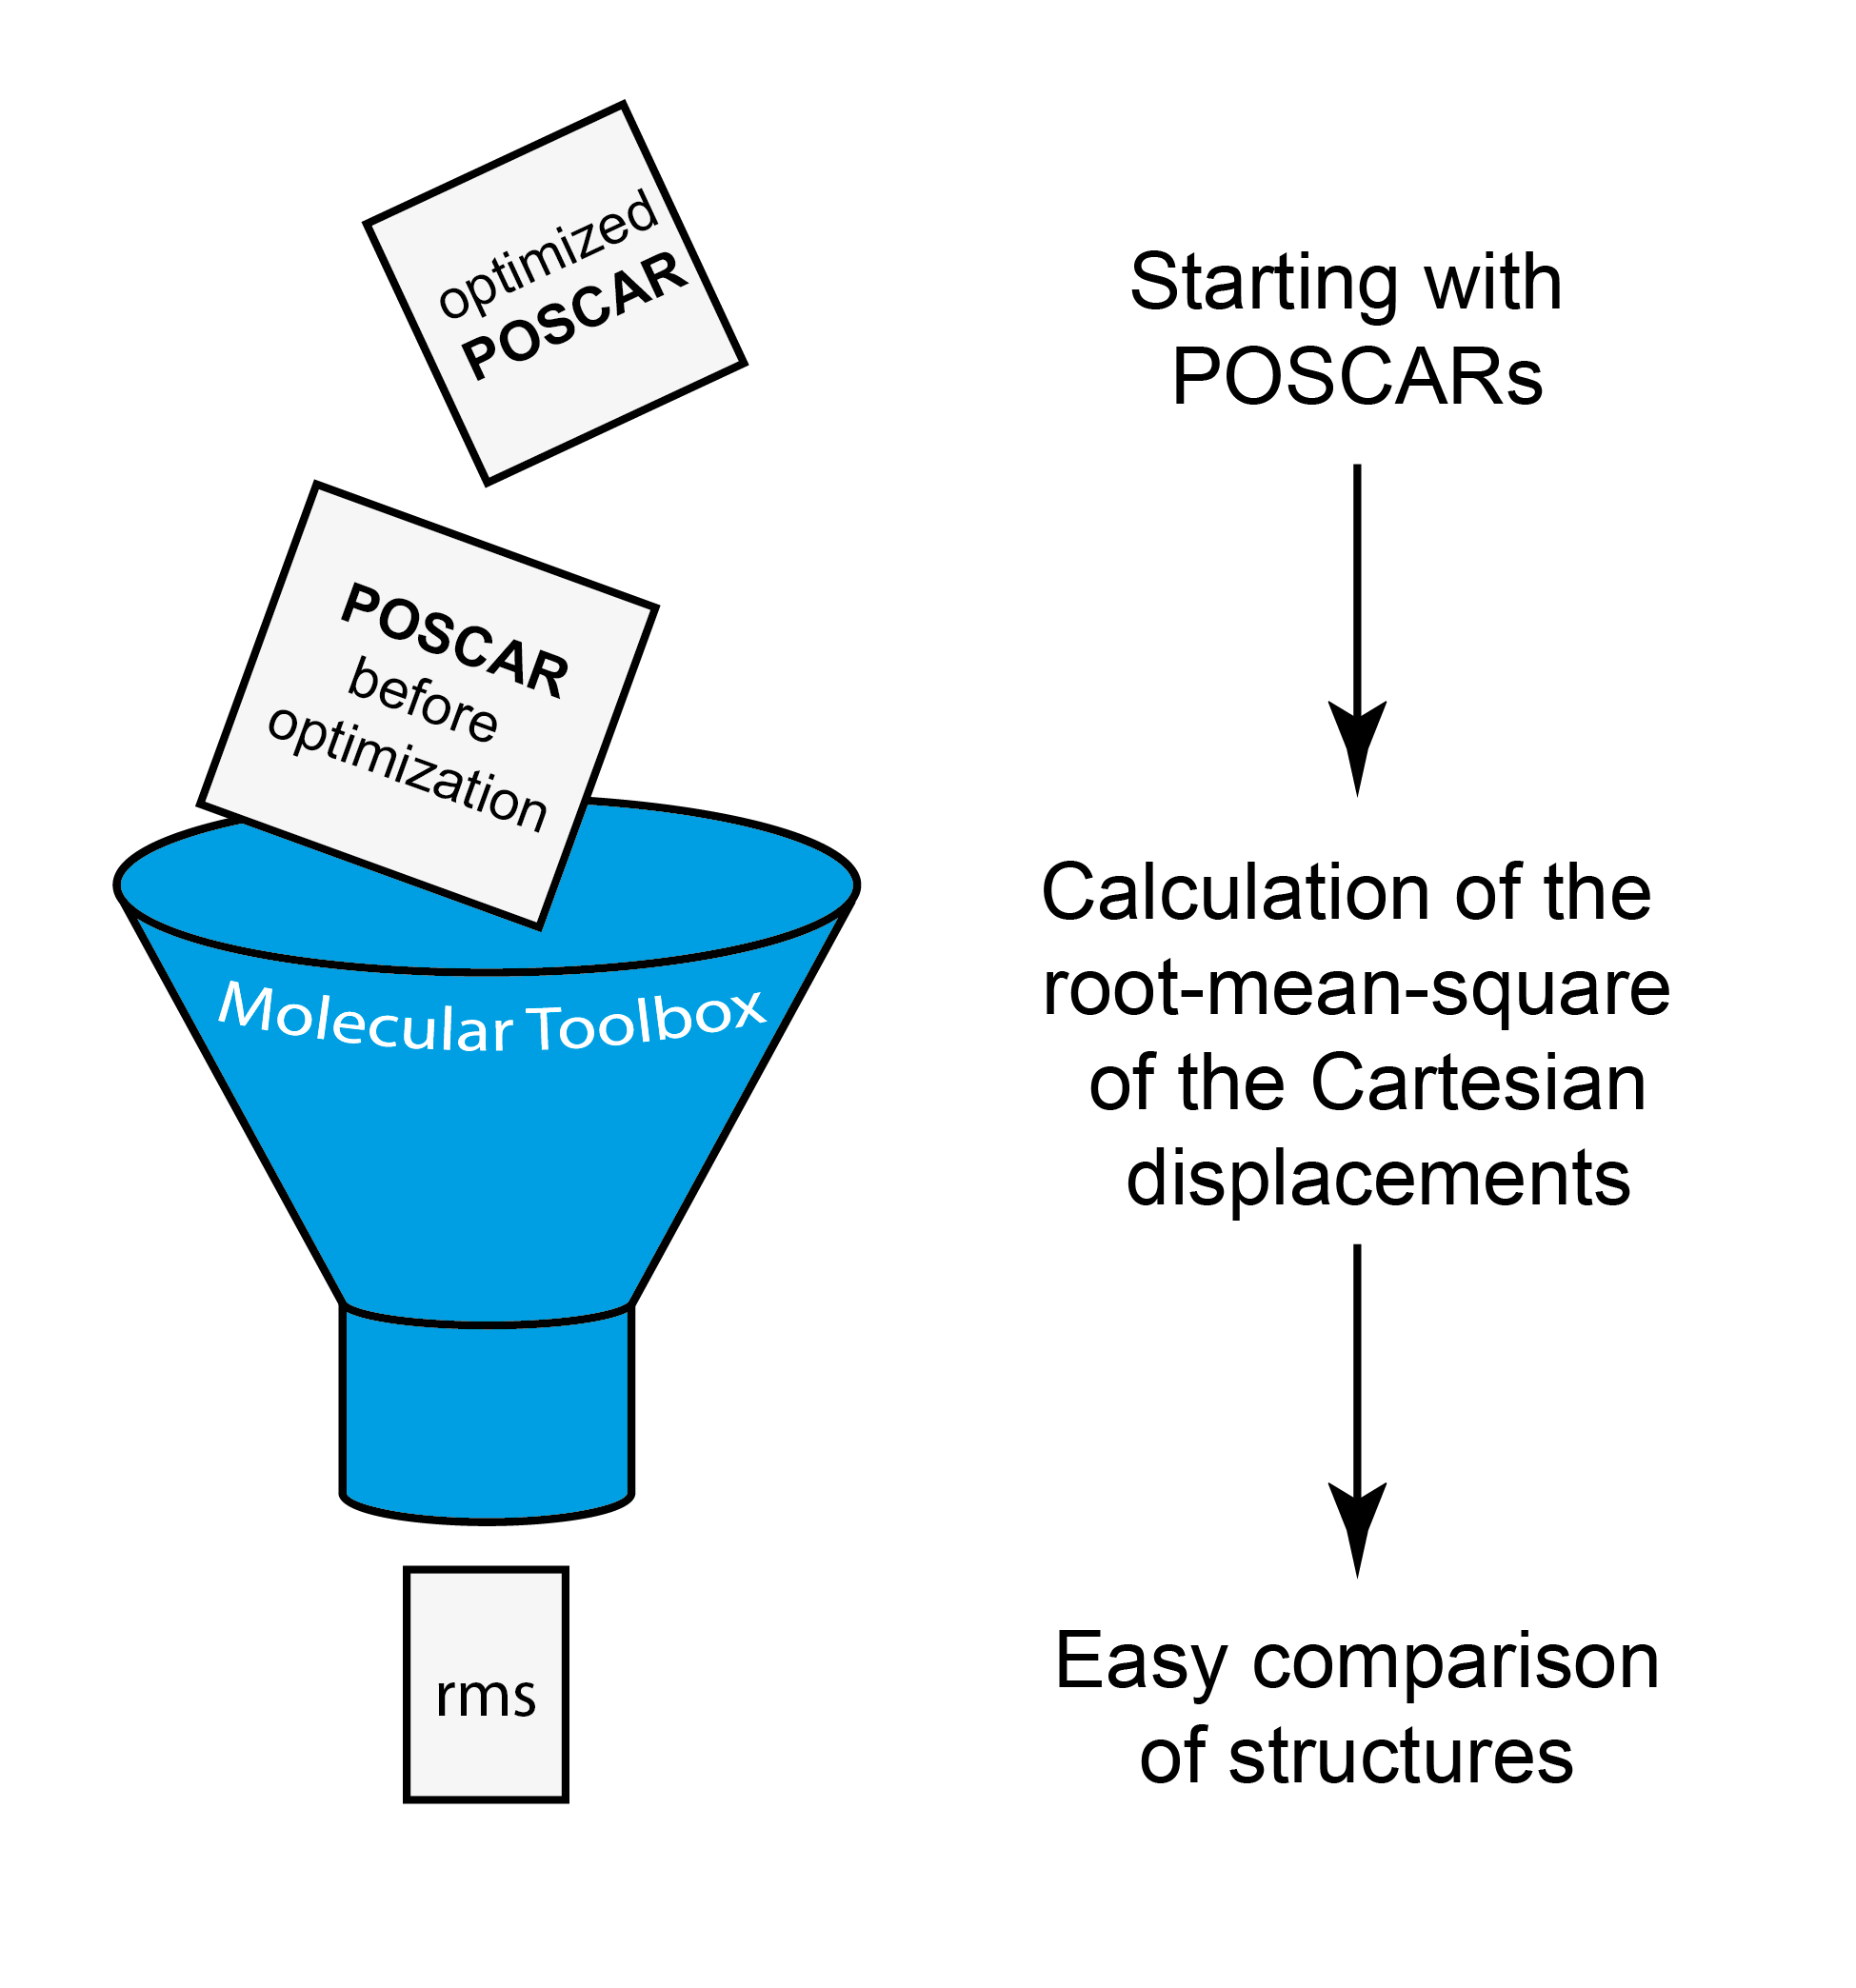
\includegraphics[width=0.4\textwidth]{Piktogramm-02.png}\end{center}
Moreover, this toolbox can also calculate the root-mean-square of the Cartesian displacements as defined in\\ J. George, V. L. Deringer, R. Dronskowski, \textit{Inorg. Chem.}, \textbf{2015}, \textit{54}, 956–962.\\   J. van de Streek, M. A. Neumann,  \textit{Acta Cryst. B}, \textbf{2010}, \textit{66},  544–558.



\newpage
\section{What to cite?}

\textbf{If you use the program to convert ADPs, please cite:}
 \begin{itemize}
  \item R. W. Grosse-Kunstleve and P. D. Adams, \textit{J. Appl. Crystallogr.}, \textbf{2002}, \textit{35}, 477–480.
  \item J. George, A. Wang, V. L. Deringer, R. Wang, R. Dronskowski, U. Englert, \textit{CrystEngComm}, \textbf{2015}, \textit{17}, 7414–7422.
 \end{itemize}
\textbf{And please, don't forget to cite Phonopy}
   \begin{itemize}
 \item A. Togo, I. Tanaka, \textit{Scr. Mater.} \textbf{2015}, \textit{108}, 1–5.
 \end{itemize}
\textbf{and the ADP calculation with Phonopy, if you have performed it:}
 \begin{itemize}
 \item V. L. Deringer, R. P. Stoffel, A. Togo, B. Eck, M. Meven, R. Dronskowski, \textit{CrystEngComm}, \textbf{2014}, \textit{16}, 10907–10915..
  \item J. George, A. Wang, V. L. Deringer, R. Wang, R. Dronskowski, U. Englert, \textit{CrystEngComm}, \textbf{2015}, \textit{17}, 7414–7422.
 \end{itemize}
 
\textbf{If you use the program to calculate the root-mean-square of the Cartesian Displacements, please cite:}
 \begin{itemize}
  \item J. George, V. L. Deringer, R. Dronskowski, \textit{Inorg. Chem.}, \textbf{2015}, \textit{54}, 956–962.
 \end{itemize}
\textbf{If you use the program to calculate the root-mean-square of the Cartesian Displacements as defined by van de Streek and Neumann, please cite:}
\begin{itemize}
  \item J. van de Streek, M. A. Neumann,  \textit{Acta Cryst. B}, \textbf{2010}, \textit{66},  544–558.
   \item J. George, V. L. Deringer, R. Dronskowski, \textit{Inorg. Chem.}, \textbf{2015}, \textit{54}, 956–962.
 \end{itemize}
  \newpage


\section{Getting Started}
\subsection{Install the MATLAB Toolbox}
\begin{enumerate}
 \item Open your MATLAB. Please use version 2015a or newer.
 \item Browse with MATLAB's explorer to the folder with the Molecular-Toolbox files.
 \item Double click on the \textbf{Molecular-Toolbox.mltbx}-file.
 \item Click \textbf{Install}.
 \item Check whether the Molecular-Toolbox is correctly installed. 
 This is done by going to the \textbf{Home} tab, then switching to the \textbf{Environment} section, clicking on the \textbf{Add-Ons} icon and finally selecting \textbf{Manage Add-Ons}.
 \item Run the scripts within the Matlab GUI or in the shell by typing: \begin{verbatim} matlab -nodisplay < NameOfTheScript.m\end{verbatim}
\end{enumerate}

\newpage
\subsection{Run the Scripts}

\subsubsection{ADPs: Starting from Phonopy Output}
In this section we explain what the script does to calculate the different parametrizations starting from the Phonopy output. 

The script is called \texttt{ConvertADPsfromPhonopy.m} and is located in the provided folder \texttt{ConvertADPsfromPhonopy}. Please have a look at the specifications of the files \texttt{POSCAR} and \texttt{thermal\_displacement\_matrices.yaml} in the chapters \ref{POSCAR} and \ref{thermal}. Make sure that you use a Phonopy version that produces the file  \texttt{thermal\_displacement\_matrices.yaml} including the anisotropic displacement parameters in the correct format.

First, the toolbox has to be imported:
\begin{lstlisting}[frame=single,language=Matlab] 
import Molecular-Toolbox.*
\end{lstlisting}


Give the pathway of the \texttt{POSCAR} file you used for the phonon calculation with Phonopy.
\begin{lstlisting}[frame=single,language=Matlab] 
FilenameOfYourPOSCAR='POSCAR';
\end{lstlisting}


Did you rename the \texttt{thermal\_displacement\_matrices.yaml}? How is it called at the moment? Make sure you used the \texttt{POSCAR} specified above to create this file.
\begin{lstlisting}[frame=single,language=Matlab] 
FilenameOfYourPhonopyADPFile='thermal_displacement_matrices.yaml';
\end{lstlisting}
Define \texttt{TMIN},\texttt{TMAX} and \texttt{TSTEP} as in the calculation with Phonopy. This is needed to read the \texttt{thermal\_displacement\_matrices.yaml} correctly.
\begin{lstlisting}[frame=single,language=Matlab] 
TMIN=0;
TMAX=300;
TSTEP=10;
\end{lstlisting}
Here, name the output files:
\begin{lstlisting}[frame=single,language=Matlab] 
CIFwithUsFilename='U.cif';
CIFwithBsFilename='B.cif';
MainAxisComponentsFilename='U1U2U3';
UstarFilename='Ustar';
BetasFilename='Betas';
UeqFilename='Ueq';
\end{lstlisting}
These are the commands to get the files written. Change these commands only if you know what you are doing!
\begin{lstlisting}[frame=single,language=Matlab] 
try
  CIF=FromPhonopywriter(FilenameOfYourPOSCAR,FilenameOfYourPhonopyADPFile,TMIN,TMAX,TSTEP);
  CIF.cifwrite(CIFwithUsFilename);
  CIF.cifwriteWithBs(CIFwithBsFilename);
  CIF.writeU1U2U3inFile(MainAxisComponentsFilename);
  CIF.writeUstarinFile(UstarFilename);
  CIF.writeBetasinFile(BetasFilename);
  CIF.writeUeqinFile(UeqFilename);
  disp('No error. All files are created :).');
catch exception
    disp(exception.message)
end
clear;
\end{lstlisting}




\subsubsection{ADPs: Starting from  $U_{\mathrm{cif}}$, $B$, $\beta$ and $U^*$}

In this section we explain what the script does to calculate various parametrizations from different ADP parametrizations. 

The scripts are called \texttt{ConvertADPsfrom*\_example.m} and are located in the folders \texttt{ConvertADPsfrom*}, the star * stands for Betas, Bs, Ucif, Ustar.

First, the toolbox has to be imported:

\begin{lstlisting}[frame=single,language=Matlab] 
import Molecular-Toolbox.*
\end{lstlisting}

Then, specify the type of input data you wish to convert. You can choose between the following keywords: \texttt{Betas}, \texttt{Bcif}, \texttt{Ucif}, \texttt{Ustar} or \texttt{Ucart}. It will only work if the spelling is correct.

\begin{lstlisting}[frame=single,language=Matlab] 
 INPUTType='Ustar';
\end{lstlisting}

Then, give the name of the input file. The tensor elements have to be sorted in the following way: \texttt{E11 E22 E33 E23 E13 E12}. It will produce incorrect results if the matrix elements are sorted differently. A sample input can be found in each of the sample folders or in chapter \ref{BetaFile}.

\begin{lstlisting}[frame=single,language=Matlab] 
 NameOfFile='UstarInput';
\end{lstlisting}

Specify the lattice parameters of the structure: $a$, $b$, $c$, $\alpha$, $\beta$, $\gamma$.
\begin{lstlisting}[frame=single,language=Matlab,] 
 a=5.350524;
 b=5.192441;
 c=15.058446;
 alpha=89.999991;
 beta=99.578013;
 gamma=89.999998;
\end{lstlisting}

Specify the temperature range by giving the starting temperature \texttt{TSTART}, the end temperature \texttt{TEND} and the step \texttt{TSTEP}.

\begin{lstlisting}[frame=single,language=Matlab] 
 TSTART=0;
 TEND=10;
 TSTEP=10;
\end{lstlisting}
Specify the number of atoms in the structure.
\begin{lstlisting}[frame=single,language=Matlab] 
 NumberofAtomsPerTemperature=22;
\end{lstlisting}

Last, name the output files here:
\begin{lstlisting}[frame=single,language=Matlab] 
 OUTPUTU1U2U3='U1U2U3';
 OUTPUTUcif='Ucif';
 OUTPUTBcif='Bcif';
 OUTPUTUstar='UstarOutput';
 OUTPUTBetas='Betas';
 OUTPUTUeq='Ueq';
\end{lstlisting}

These are the commands to get the files written. Change these commands only if you know what you are doing.
\begin{lstlisting}[frame=single,language=Matlab] 
try
  if strcmp(INPUTType,'Bcif')
    NewWriter=FromBcifwriter(a,b,c,alpha,beta,gamma,NameOfFile,TSTART,TEND,TSTEP,NumberofAtomsPerTemperature);
  elseif  strcmp(INPUTType,'Betas')
    NewWriter=FromBetaswriter(a,b,c,alpha,beta,gamma,NameOfFile,TSTART,TEND,TSTEP,NumberofAtomsPerTemperature);
  elseif strcmp(INPUTType,'Ucif')
    NewWriter=FromUcifwriter(a,b,c,alpha,beta,gamma,NameOfFile,TSTART,TEND,TSTEP,NumberofAtomsPerTemperature);
  elseif strcmp(INPUTType,'Ustar')
    NewWriter=FromUstarwriter(a,b,c,alpha,beta,gamma,NameOfFile,TSTART,TEND,TSTEP,NumberofAtomsPerTemperature);
  end

  NewWriter.writeU1U2U3inFile(OUTPUTU1U2U3);
  NewWriter.writeUcifinFile(OUTPUTUcif);
  NewWriter.writeBcifinFile(OUTPUTBcif);
  NewWriter.writeUstarinFile(OUTPUTUstar);
  NewWriter.writeBetasinFile(OUTPUTBetas);
  NewWriter.writeUeqinFile(OUTPUTUeq);
  disp('No error. All files are created :).');
catch exception
    disp(exception.message)
end
clear;
\end{lstlisting}



    


\subsubsection{RMS of the Cartesian Displacements}
This section explains how the root-mean-square of the Cartesian displacements is calculated. The script is called \texttt{CalculateRMS.m} and lies in the folder \texttt{CalculateRMS}.

First, the toolbox has to be imported:

\begin{lstlisting}[frame=single,language=Matlab] 
import Molecular-Toolbox.*
\end{lstlisting}
The script does not work if the atoms of the two \texttt{POSCAR}s are sorted differently!

Just define the relative pathways of the sorted \texttt{POSCAR}s and the output file below. Then run the script.
\begin{lstlisting}[frame=single,language=Matlab] 
PathwayPOSCAR1='POSCAR.vdw';
PathwayPOSCAR2='POSCAR_exp100K';
filenameOUTPUT='RMS';
\end{lstlisting}
If you do not know what you are doing, do not change anything here, please.
\begin{lstlisting}[frame=single,language=Matlab] 
try
  RMS1=RMS(PathwayPOSCAR1,PathwayPOSCAR2);
  RMS1.printFileRMSandRMSxyz(filenameOUTPUT);
  disp('No error. All files are created :).');
catch exception
    disp(exception.message)
end
clear;
\end{lstlisting}


  


\newpage
 \section{Requirements for the INPUT files}
 
 \subsection{POSCAR}\label{POSCAR}
 
\textbf{A sample POSCAR:}
\begin{lstlisting}[frame=single] 
 This is a sample POSCAR
    1.00000000000000
     5.3505    0.0000    0.0097
    -0.0000    5.1924    0.0000
    -2.5327    0.0000   14.8439
   Cl   C    N
    10    10     2
Direct
  0.1149  0.6767  0.3328
  0.1149  0.3232  0.8328
  0.5321  0.1092  0.3241
  0.5321  0.8907  0.8241
  0.9618  0.1771  0.4921
  0.9618  0.8228  0.9921
  0.9686  0.8162  0.6599
  0.9686  0.1837  0.1599
  0.5316  0.3970  0.6530
  0.5316  0.6029  0.1530
  0.3582  0.7256  0.4215
  0.3582  0.2743  0.9215
  0.5410  0.9176  0.4169
  0.5410  0.0823  0.9169
  0.5430  0.6026  0.5637
  0.5430  0.3973  0.0637
  0.7340  0.9476  0.4921
  0.7340  0.0523  0.9921
  0.7373  0.7867  0.5677
  0.7373  0.2132  0.0677
  0.3619  0.5754  0.4928
  0.3619  0.4245  0.9928
\end{lstlisting}
\textbf{Requirements}
\begin{itemize}
  \item The scaling factor is not allowed to be smaller than 0.0 or equal to 0.0 (line 2).
  \item The names of the elements have to be included (line 6 of the sample \texttt{POSCAR}).
  \item No \texttt{Selective Dynamics} are allowed.
  \item Only \texttt{direct} coordinates are allowed (lines 8--30).
  \item If you calculate the RMS of the Cartesian displacements, the atoms in the two \texttt{POSCAR}s have to be sorted in the same way!
  \item If you have other questions about this format, please read the VASP documentation (\url{http://www.vasp.at}).
 \end{itemize}
 
  \newpage
 \subsection{thermal\_displacement\_matrices.yaml}\label{thermal}
   \textbf{Sample thermal\_displacement\_matrices.yaml ($\mathbf{\geq}$ Phonopy Version 1.11.2)}
 \begin{lstlisting}[
 basicstyle=\small,
 ]
  # Thermal displacement_matrices
natom:    22
cutoff_frequency: 0.130000
thermal_displacement_matrices:
- temperature:         0.0000000
  displacement_matrices:
  - [  0.00516,  0.00613,  0.00415, -0.00011, -0.00158, -0.00081 ] # atom 1
  - [  0.00612,  0.00548,  0.00395,  0.00157, -0.00013, -0.00079 ] # atom 2
  - [  0.00420,  0.00425,  0.00533,  0.00000, -0.00003, -0.00139 ] # atom 3
  - [  0.00518,  0.00633,  0.00394,  0.00014, -0.00152, -0.00068 ] # atom 4
  - [  0.00616,  0.00522,  0.00414,  0.00153,  0.00010, -0.00089 ] # atom 5
  - [  0.00516,  0.00613,  0.00415,  0.00011, -0.00158,  0.00081 ] # atom 6
  - [  0.00612,  0.00548,  0.00395, -0.00157, -0.00013,  0.00079 ] # atom 7
  - [  0.00420,  0.00425,  0.00533, -0.00000, -0.00003,  0.00139 ] # atom 8
  - [  0.00518,  0.00633,  0.00394, -0.00014, -0.00152,  0.00068 ] # atom 9
  - [  0.00616,  0.00522,  0.00414, -0.00153,  0.00010,  0.00089 ] # atom 10
  - [  0.00427,  0.00451,  0.00370,  0.00032, -0.00059, -0.00083 ] # atom 11
  - [  0.00438,  0.00444,  0.00365,  0.00059, -0.00042, -0.00086 ] # atom 12
  - [  0.00446,  0.00433,  0.00370,  0.00057, -0.00033, -0.00083 ] # atom 13
  - [  0.00413,  0.00419,  0.00381,  0.00037, -0.00039, -0.00090 ] # atom 14
  - [  0.00433,  0.00444,  0.00365,  0.00041, -0.00059, -0.00082 ] # atom 15
  - [  0.00427,  0.00451,  0.00370, -0.00032, -0.00059,  0.00083 ] # atom 16
  - [  0.00438,  0.00444,  0.00365, -0.00059, -0.00042,  0.00086 ] # atom 17
  - [  0.00446,  0.00433,  0.00370, -0.00057, -0.00033,  0.00083 ] # atom 18
  - [  0.00413,  0.00419,  0.00381, -0.00037, -0.00039,  0.00090 ] # atom 19
  - [  0.00433,  0.00444,  0.00365, -0.00041, -0.00059,  0.00082 ] # atom 20
  - [  0.00488,  0.00497,  0.00397,  0.00070, -0.00070, -0.00144 ] # atom 21
  - [  0.00488,  0.00497,  0.00397, -0.00070, -0.00070,  0.00144 ] # atom 22
  displacement_matrices_cif:
  - [  0.00457,  0.00613,  0.00415, -0.00011, -0.00081, -0.00082 ] # atom 1
  - [  0.00601,  0.00548,  0.00395,  0.00157,  0.00058, -0.00049 ] # atom 2
  - [  0.00423,  0.00425,  0.00533,  0.00000,  0.00092, -0.00136 ] # atom 3
  - [  0.00460,  0.00633,  0.00394,  0.00014, -0.00080, -0.00065 ] # atom 4
  - [  0.00613,  0.00522,  0.00414,  0.00153,  0.00083, -0.00061 ] # atom 5
  - [  0.00457,  0.00613,  0.00415,  0.00011, -0.00081,  0.00082 ] # atom 6
  - [  0.00601,  0.00548,  0.00395, -0.00157,  0.00058,  0.00049 ] # atom 7
  - [  0.00423,  0.00425,  0.00533, -0.00000,  0.00092,  0.00136 ] # atom 8
  - [  0.00460,  0.00633,  0.00394, -0.00014, -0.00080,  0.00065 ] # atom 9
  - [  0.00613,  0.00522,  0.00414, -0.00153,  0.00083,  0.00061 ] # atom 10
  - [  0.00405,  0.00451,  0.00370,  0.00032,  0.00008, -0.00076 ] # atom 11
  - [  0.00421,  0.00444,  0.00365,  0.00059,  0.00024, -0.00074 ] # atom 12
  - [  0.00432,  0.00433,  0.00370,  0.00057,  0.00033, -0.00071 ] # atom 13
  - [  0.00399,  0.00419,  0.00381,  0.00037,  0.00030, -0.00082 ] # atom 14
  - [  0.00410,  0.00444,  0.00365,  0.00041,  0.00007, -0.00074 ] # atom 15
  - [  0.00405,  0.00451,  0.00370, -0.00032,  0.00008,  0.00076 ] # atom 16
  - [  0.00421,  0.00444,  0.00365, -0.00059,  0.00024,  0.00074 ] # atom 17
  - [  0.00432,  0.00433,  0.00370, -0.00057,  0.00033,  0.00071 ] # atom 18
  - [  0.00399,  0.00419,  0.00381, -0.00037,  0.00030,  0.00082 ] # atom 19
  - [  0.00410,  0.00444,  0.00365, -0.00041,  0.00007,  0.00074 ] # atom 20
  - [  0.00461,  0.00497,  0.00397,  0.00070,  0.00002, -0.00129 ] # atom 21
  - [  0.00461,  0.00497,  0.00397, -0.00070,  0.00002,  0.00129 ] # atom 22  
 \end{lstlisting}

 
 \newpage
\textbf{Sample thermal\_displacement\_matrices.yaml ($\mathbf{\leq}$ Phonopy Version 1.11.1)}
 \begin{lstlisting}[
 basicstyle=\small,
 ]
# Thermal displacement_matrices
natom:    22
cutoff_frequency: 0.130000
thermal_displacement_matrices:
- temperature:         0.0000000
  displacement_matrices:
  - [ 0.005083, 0.006011, 0.004118, -0.000079, -0.001577, -0.000813 ] # atom 1
  - [ 0.005083, 0.006011, 0.004118,  0.000079, -0.001577,  0.000813 ] # atom 2
  - [ 0.006039, 0.005437, 0.003949,  0.001616, -0.000284, -0.000838 ] # atom 3
  - [ 0.006039, 0.005437, 0.003949, -0.001616, -0.000284,  0.000838 ] # atom 4
  - [ 0.004167, 0.004238, 0.005192,  0.000015, -0.000068, -0.001359 ] # atom 5
  - [ 0.004167, 0.004238, 0.005192, -0.000015, -0.000068,  0.001359 ] # atom 6
  - [ 0.005127, 0.006339, 0.003925,  0.000279, -0.001566, -0.000697 ] # atom 7
  - [ 0.005127, 0.006339, 0.003925, -0.000279, -0.001566,  0.000697 ] # atom 8
  - [ 0.006152, 0.005091, 0.004119,  0.001507,  0.000065, -0.000875 ] # atom 9
  - [ 0.006152, 0.005091, 0.004119, -0.001507,  0.000065,  0.000875 ] # atom 10
  - [ 0.004275, 0.004507, 0.003681,  0.000350, -0.000623, -0.000852 ] # atom 11
  - [ 0.004275, 0.004507, 0.003681, -0.000350, -0.000623,  0.000852 ] # atom 12
  - [ 0.004361, 0.004422, 0.003636,  0.000622, -0.000489, -0.000861 ] # atom 13
  - [ 0.004361, 0.004422, 0.003636, -0.000622, -0.000489,  0.000861 ] # atom 14
  - [ 0.004474, 0.004318, 0.003685,  0.000601, -0.000371, -0.000833 ] # atom 15
  - [ 0.004474, 0.004318, 0.003685, -0.000601, -0.000371,  0.000833 ] # atom 16
  - [ 0.004111, 0.004176, 0.003762,  0.000408, -0.000442, -0.000887 ] # atom 17
  - [ 0.004111, 0.004176, 0.003762, -0.000408, -0.000442,  0.000887 ] # atom 18
  - [ 0.004316, 0.004425, 0.003633,  0.000461, -0.000630, -0.000810 ] # atom 19
  - [ 0.004316, 0.004425, 0.003633, -0.000461, -0.000630,  0.000810 ] # atom 20
  - [ 0.004931, 0.004991, 0.003964,  0.000758, -0.000766, -0.001472 ] # atom 21
  - [ 0.004931, 0.004991, 0.003964, -0.000758, -0.000766,  0.001472 ] # atom 22
 \end{lstlisting}
 
\textbf{Requirements}
\begin{itemize}
 \item Please make sure that you used the specified \texttt{POSCAR} to calculate the matrices!
\end{itemize}

 \newpage
 \subsection{Reading in $U_{\mathrm{cif}}$, $U^*$, $B$, $\beta$, $U_{\mathrm{cart}}$}\label{BetaFile}
Sample file for reading in $\beta$s:
\begin{lstlisting}[
 basicstyle=\small,
 ]
0 
Cl1  0.003214 0.004401 0.000369 -0.000020 -0.000219 -0.000587
Cl2  0.003214 0.004401 0.000369  0.000020 -0.000219  0.000587
Cl3  0.004174 0.003981 0.000354  0.000414  0.000094 -0.000399
Cl4  0.004174 0.003981 0.000354 -0.000414  0.000094  0.000399
Cl5  0.002960 0.003103 0.000465  0.000004  0.000201 -0.000963
Cl6  0.002960 0.003103 0.000465 -0.000004  0.000201  0.000963
Cl7  0.003243 0.004641 0.000352  0.000072 -0.000225 -0.000461
Cl8  0.003243 0.004641 0.000352 -0.000072 -0.000225  0.000461
Cl9  0.004337 0.003727 0.000369  0.000386  0.000188 -0.000439
Cl10 0.004337 0.003727 0.000369 -0.000386  0.000188  0.000439
C1   0.002873 0.003300 0.000330  0.000090 -0.000001 -0.000563
C2   0.002873 0.003300 0.000330 -0.000090 -0.000001  0.000563
C3   0.002963 0.003237 0.000326  0.000160  0.000031 -0.000536
C4   0.002963 0.003237 0.000326 -0.000160  0.000031  0.000536
C5   0.003070 0.003161 0.000330  0.000154  0.000062 -0.000519
C6   0.003070 0.003161 0.000330 -0.000154  0.000062  0.000519
C7   0.002804 0.003057 0.000337  0.000105  0.000048 -0.000581
C8   0.002804 0.003057 0.000337 -0.000105  0.000048  0.000581
C9   0.002899 0.003240 0.000325  0.000118 -0.000004 -0.000519
C10  0.002899 0.003240 0.000325 -0.000118 -0.000004  0.000519
N1   0.003297 0.003654 0.000355  0.000195 -0.000024 -0.000954
N2   0.003297 0.003654 0.000355 -0.000195 -0.000024  0.000954
 \end{lstlisting}

 \begin{itemize}
  \item First, the temperature is given (line 1).
  \item Then (lines 2--23, in this case), the tensor elements are given in the following order in each line after the name of the atom (e.g. Cl1):\\ $\beta_{11}$ $\beta_{22}$ $\beta_{33}$ $\beta_{23}$ $\beta_{13}$ $\beta_{12}$ 
  \item You could start with another temperature and tensor elements of the same structure in line 24.
 \end{itemize}
 \textbf{Warning: If you don't use the order of the tensor elements described above, your results will be wrong!}
 \newpage
 \section{Output files}
 \subsection{ADPs: Starting from Phonopy Output}
 These are the files you will get:
 \begin{itemize}
  \item A CIF file in $P1$ space group including $U_{\mathrm{cif}}$
  \item A CIF file in $P1$ space group including $B$
  \item A file containing the main-axis components $U_1$, $U_2$, $U_3$
  \item A file containing $U_{eq}$
  \item Files containing the tensor elements of $\beta$ and $U^*$
  
 \end{itemize}

 
 
 \subsection{ADPs: Starting from $U_{\mathrm{cif}}$, $B$, $\beta$, $U^*$ and $U_{\mathrm{cart}}$}
 These are the files you will get:
\begin{itemize}
 \item A file containing the main-axis components $U_1$, $U_2$, $U_3$
  \item A file containing $U_{eq}$
  \item Files containing the tensor elements of $U_{\mathrm{cif}}$, $B$, $\beta$ and $U^*$
  \end{itemize}
 \subsection{RMS of the Cartesian Displacements}
  \begin{itemize}
 \item The file contains the rms, rms$_x$, rms$_y$ and rms$_z$ for all atoms and for each atom type as defined by George et al. 
 \item The file also contains the rms as defined by van de Streek and Neumann
  \end{itemize}
 \newpage
 
 \section{Version history}
 
 \begin{center}
\begin{tabular}{|l|l|}\hline
1.0.0 (February 2016)& First Molecular-Toolbox version is released! \\ \hline
1.0.1 (September 2016)& Compatible with Phonopy 1.11.2.\\ \hline
1.0.2 (April 2017) & RMS of van de Streek and Neumann is included \\
                   & Further safety checks are included in the RMS calculation \\
                   & ADP transformation starting from $U_{\mathrm{cart}}$ is included \\  \hline           
 \end{tabular}
 \end{center}

 \newpage
\section{License of the Molecular Toolbox: BSD 3-Clause License}

\begin{framed}\raggedright{Copyright (c) 2015--2017, Janine George

All rights reserved.

Redistribution and use in source and binary forms, with or without modification, are permitted provided that the following conditions are met:

1. Redistributions of source code must retain the above copyright notice, this list of conditions and the following disclaimer.

2. Redistributions in binary form must reproduce the above copyright notice, this list of conditions and the following disclaimer in the documentation and/or other materials provided with the distribution.

3. Neither the name of the copyright holder nor the names of its contributors may be used to endorse or promote products derived from this software without specific prior written permission.

THIS SOFTWARE IS PROVIDED BY THE COPYRIGHT HOLDERS AND CONTRIBUTORS "AS IS" AND ANY EXPRESS OR IMPLIED WARRANTIES, INCLUDING, BUT NOT LIMITED TO, THE IMPLIED WARRANTIES OF MERCHANTABILITY AND FITNESS FOR A PARTICULAR PURPOSE ARE DISCLAIMED. IN NO EVENT SHALL THE COPYRIGHT HOLDER OR CONTRIBUTORS BE LIABLE FOR ANY DIRECT, INDIRECT, INCIDENTAL, SPECIAL, EXEMPLARY, OR CONSEQUENTIAL DAMAGES (INCLUDING, BUT NOT LIMITED TO, PROCUREMENT OF SUBSTITUTE GOODS OR SERVICES; LOSS OF USE, DATA, OR PROFITS; OR BUSINESS INTERRUPTION) HOWEVER CAUSED AND ON ANY THEORY OF LIABILITY, WHETHER IN CONTRACT, STRICT LIABILITY, OR TORT (INCLUDING NEGLIGENCE OR OTHERWISE) ARISING IN ANY WAY OUT OF THE USE OF THIS SOFTWARE, EVEN IF ADVISED OF THE POSSIBILITY OF SUCH DAMAGE.}\end{framed}


\newpage
 %\listoftodos 
 
\end{document}
